%%%%%%%%%%%%%%%%%%%%%%%%%%%%%%%%%%%%%%%%%%%%%%%%%%%%%%%%%%%%%%%%%%%%%%%%%%%%%%%%%%%%%%%%%%%%%%%%
%
% CS484 Written Question Template
%
% Acknowledgements:
% The original code is written by Prof. James Tompkin (james_tompkin@brown.edu).
% The second version is revised by Prof. Min H. Kim (minhkim@kaist.ac.kr).
%
% This is a LaTeX document. LaTeX is a markup language for producing 
% documents. Your task is to fill out this document, then to compile 
% it into a PDF document. 
%
% 
% TO COMPILE:
% > pdflatex thisfile.tex
%
% If you do not have LaTeX and need a LaTeX distribution:
% - Personal laptops (all common OS): www.latex-project.org/get/
% - We recommend latex compiler miktex (https://miktex.org/) for windows,
%   macTex (http://www.tug.org/mactex/) for macOS users.
%   And TeXstudio(http://www.texstudio.org/) for latex editor.
%   You should install both compiler and editor for editing latex.
%   The another option is Overleaf (https://www.overleaf.com/) which is 
%   an online latex editor.
%
% If you need help with LaTeX, please come to office hours. 
% Or, there is plenty of help online:
% https://en.wikibooks.org/wiki/LaTeX
%
% Good luck!
% Min and the CS484 staff
%
%%%%%%%%%%%%%%%%%%%%%%%%%%%%%%%%%%%%%%%%%%%%%%%%%%%%%%%%%%%%%%%%%%%%%%%%%%%%%%%%%%%%%%%%%%%%%%%%
%
% How to include two graphics on the same line:
% 
% \includegraphics[width=0.49\linewidth]{yourgraphic1.png}
% \includegraphics[width=0.49\linewidth]{yourgraphic2.png}
%
% How to include equations:
%
% \begin{equation}
% y = mx+c
% \end{equation}
% 
%%%%%%%%%%%%%%%%%%%%%%%%%%%%%%%%%%%%%%%%%%%%%%%%%%%%%%%%%%%%%%%%%%%%%%%%%%%%%%%%%%%%%%%%%%%%%%%%

\documentclass[11pt]{article}

\usepackage[english]{babel}
\usepackage[utf8]{inputenc}
\usepackage[colorlinks = true,
            linkcolor = blue,
            urlcolor  = blue]{hyperref}
\usepackage[a4paper,margin=1.5in]{geometry}
\usepackage{stackengine,graphicx}
\usepackage{fancyhdr}
\setlength{\headheight}{15pt}
\usepackage{microtype}
\usepackage{times}

% From https://ctan.org/pkg/matlab-prettifier
\usepackage[numbered,framed]{matlab-prettifier}

\frenchspacing
\setlength{\parindent}{0cm} % Default is 15pt.
\setlength{\parskip}{0.3cm plus1mm minus1mm}

\pagestyle{fancy}
\fancyhf{}
\lhead{Homework 3 Questions}
\rhead{CS 484}
\rfoot{\thepage}

\date{}

\title{\vspace{-1cm}Homework 3 Questions}


\begin{document}
\maketitle
\vspace{-3cm}
\thispagestyle{fancy}

\section*{Instructions}
\begin{itemize}
  \item 4 questions.
  \item Write code where appropriate.
  \item Feel free to include images or equations.
  \item Please make this document anonymous.
  \item \textbf{Please use only the space provided and keep the page breaks.} Please do not make new pages, nor remove pages. The document is a template to help grading.
  \item If you really need extra space, please use new pages at the end of the document and refer us to it in your answers.
\end{itemize}

\section*{Questions}

\paragraph{Q1:} Imagine we were tasked with designing a feature point which could match all of the following three pairs of images. Which real world phenomena and camera effects might cause us problems?
Use the MATLAB function \href{https://www.mathworks.com/help/images/ref/corner.html}{$corner$} to investigate. $corner(I,1000)$.

\emph{RISHLibrary} | \emph{Chase} | \emph{LaddObservatory}

%%%%%%%%%%%%%%%%%%%%%%%%%%%%%%%%%%%
\paragraph{A1:} Your answer here.

In the case of \textit{RISHLibrary}, we can see that the feature detected in the first picture follows the pattern of the floor, 
but there cannot be observed much pattern-following feature points in second picture. It seems that the tone of light could affect the feature detection.

In the case of \textit{Chase}, we can see that the second picture cannot be detected the eye of the object, while first picture could.
This result is thought to be occurred because of the camera shivering.

In the case of \textit{LaddObservatory}, the features detected at the first picture show us the pattern of the bricks. But in the second picture, we could not find the brick features that much.
The scale of the objects described in the picture may affect the feature detection.

\begin{figure}[!hp]
  \centering
  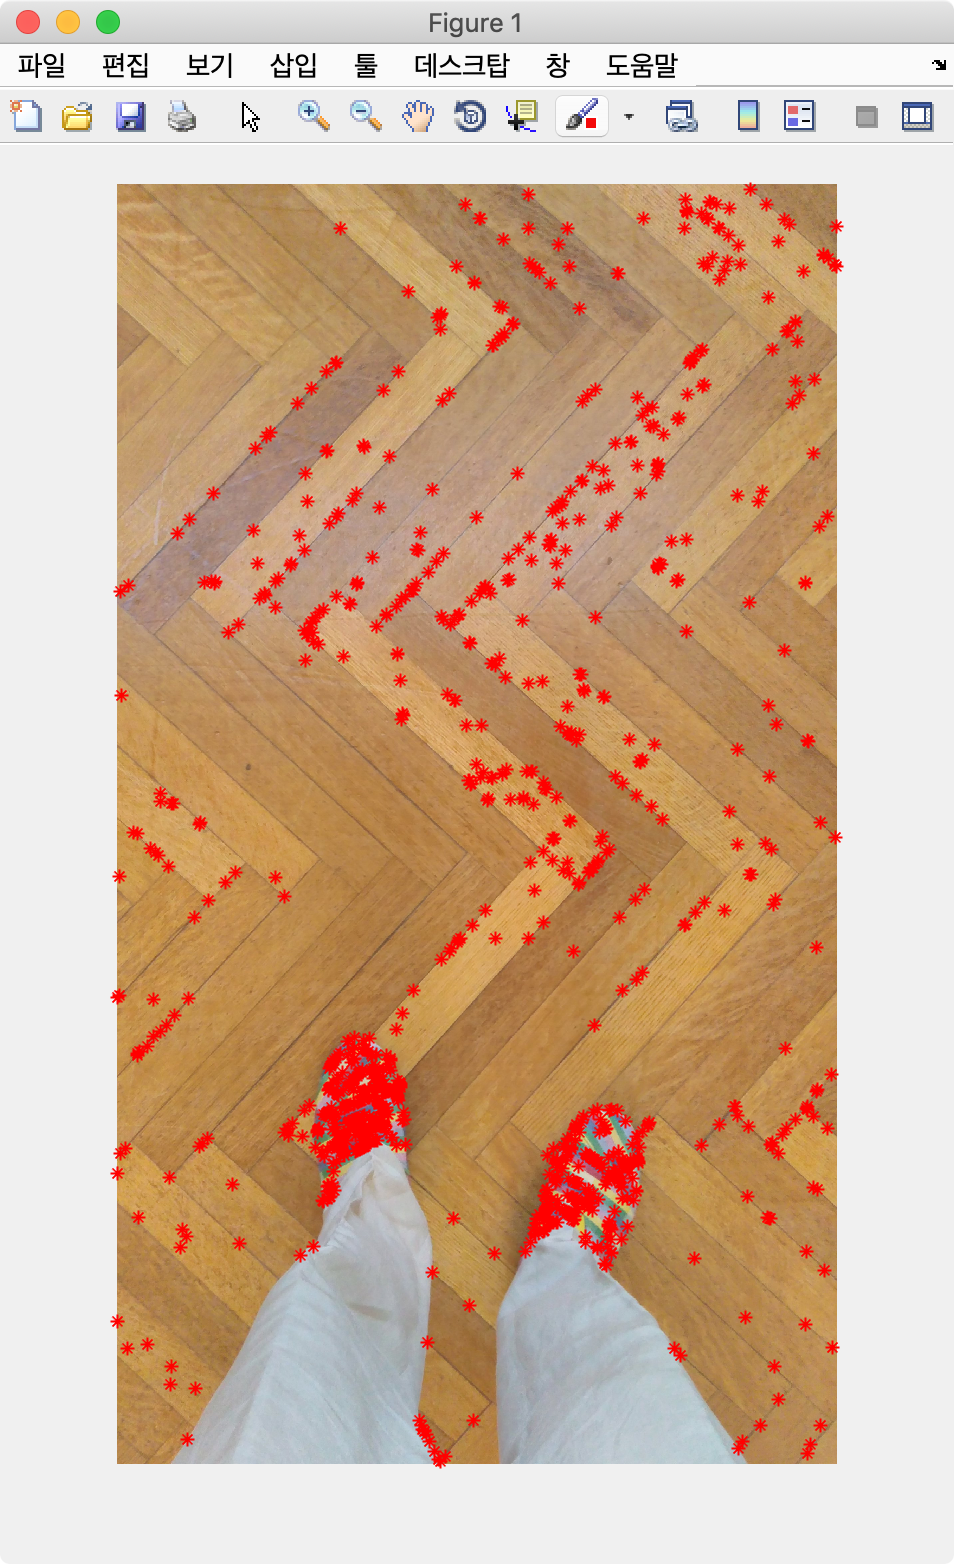
\includegraphics[width=3cm]{ri1.png}
  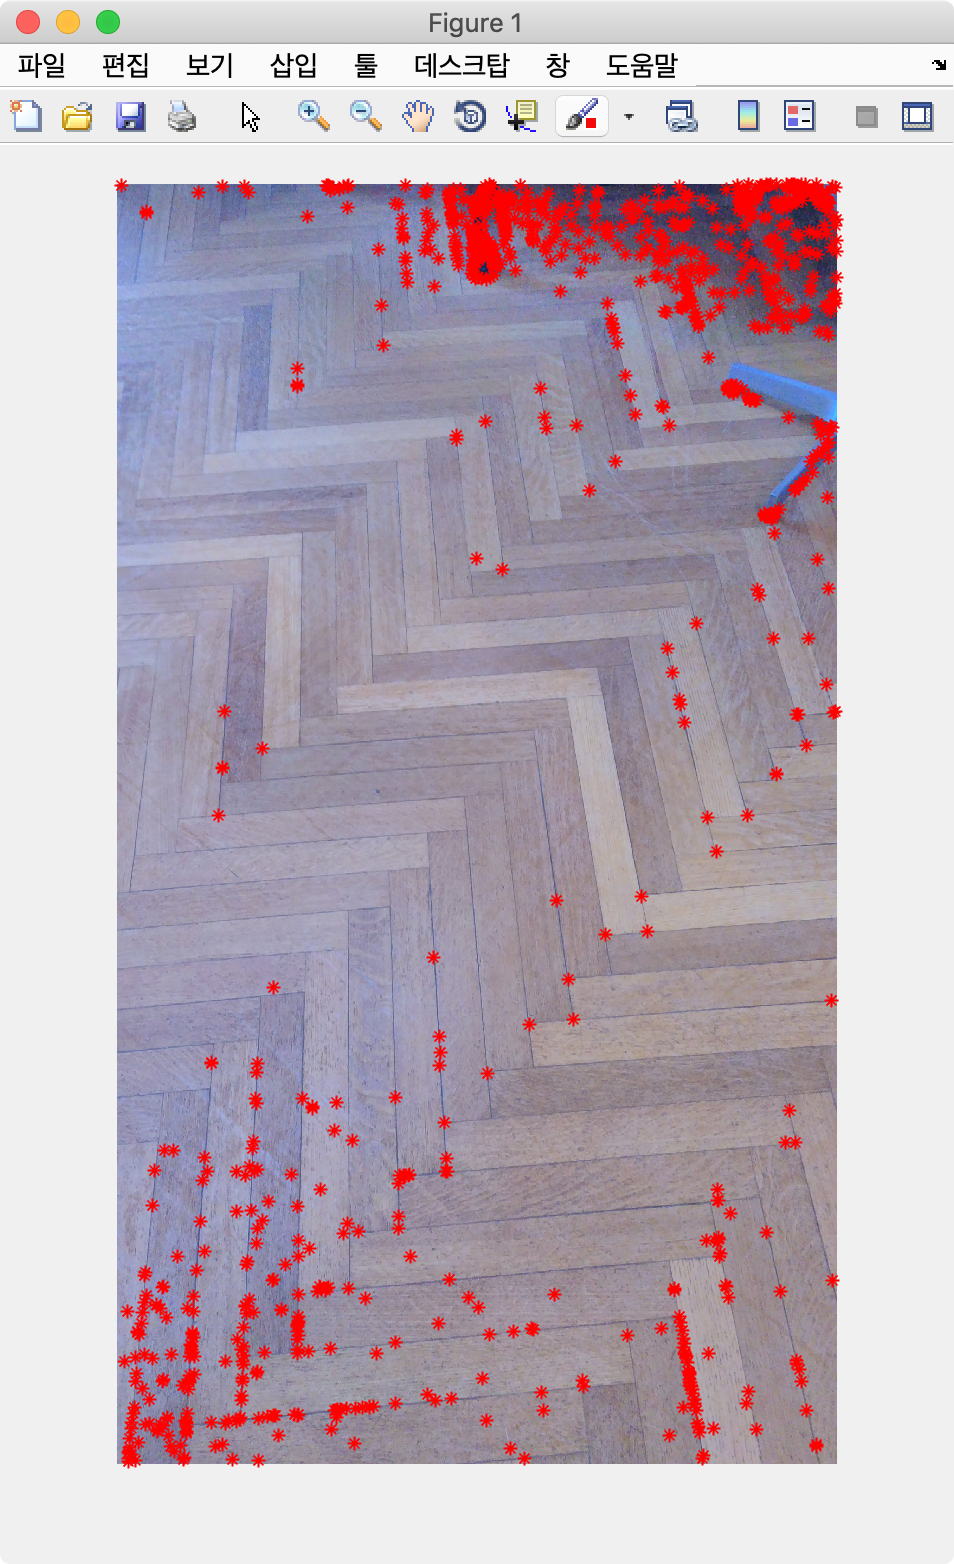
\includegraphics[width=3cm]{ri2.png}
  \caption{Result of \textit{RISHLibrary}}
  \label{fig:RISHLibrary}
\end{figure}

\begin{figure}[!hp]
  \centering
  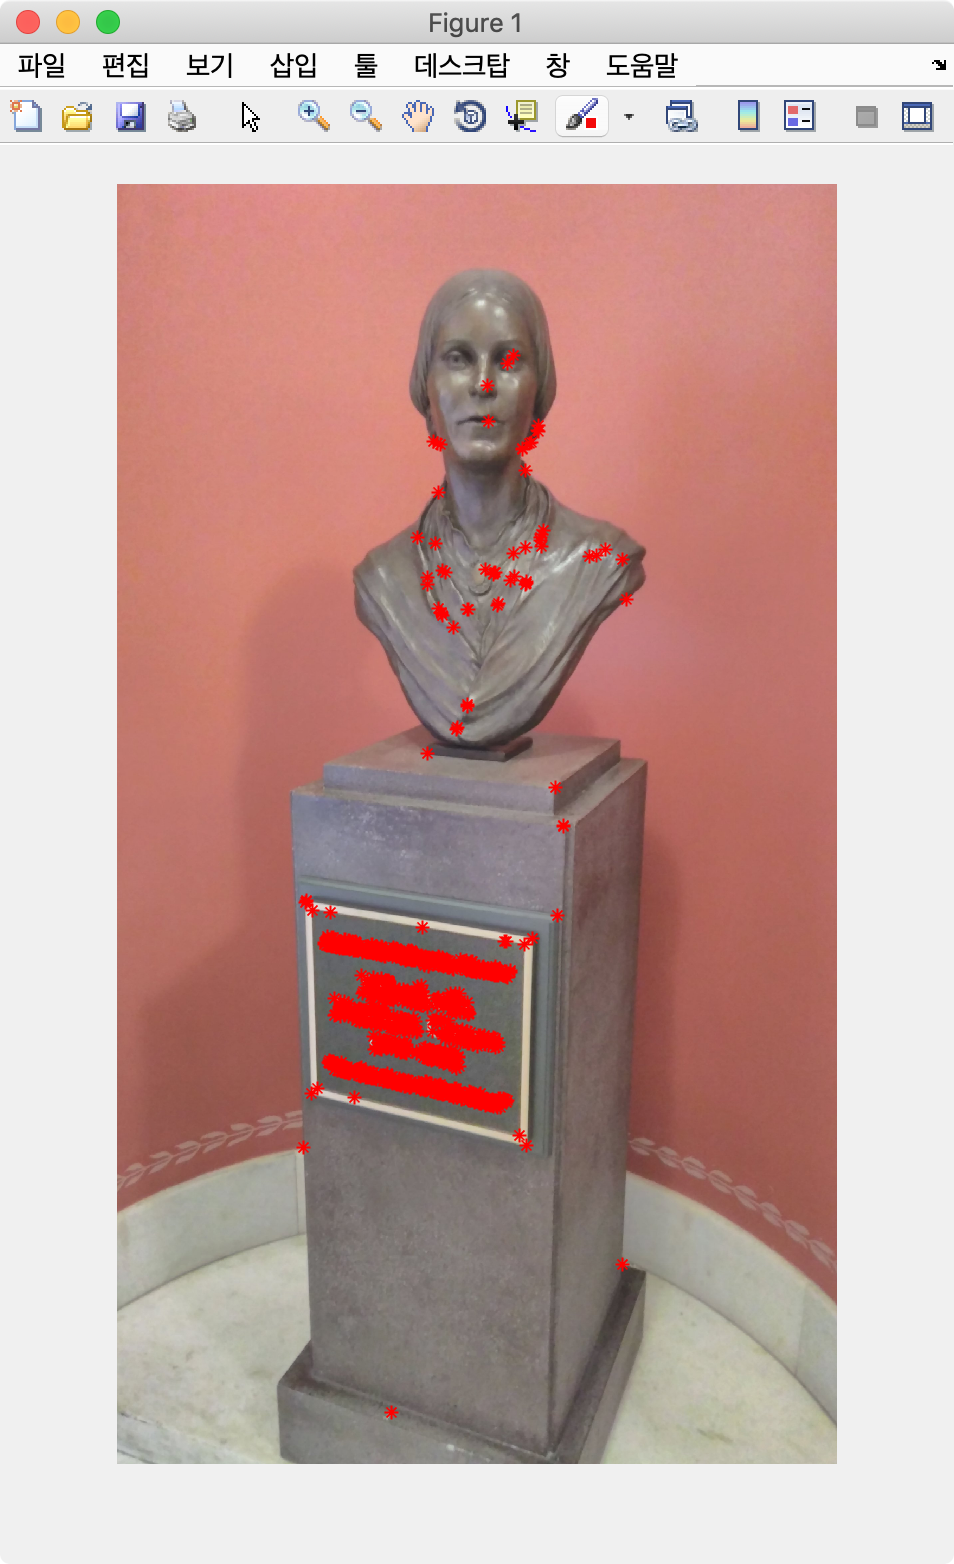
\includegraphics[width=3cm]{ch1.png}
  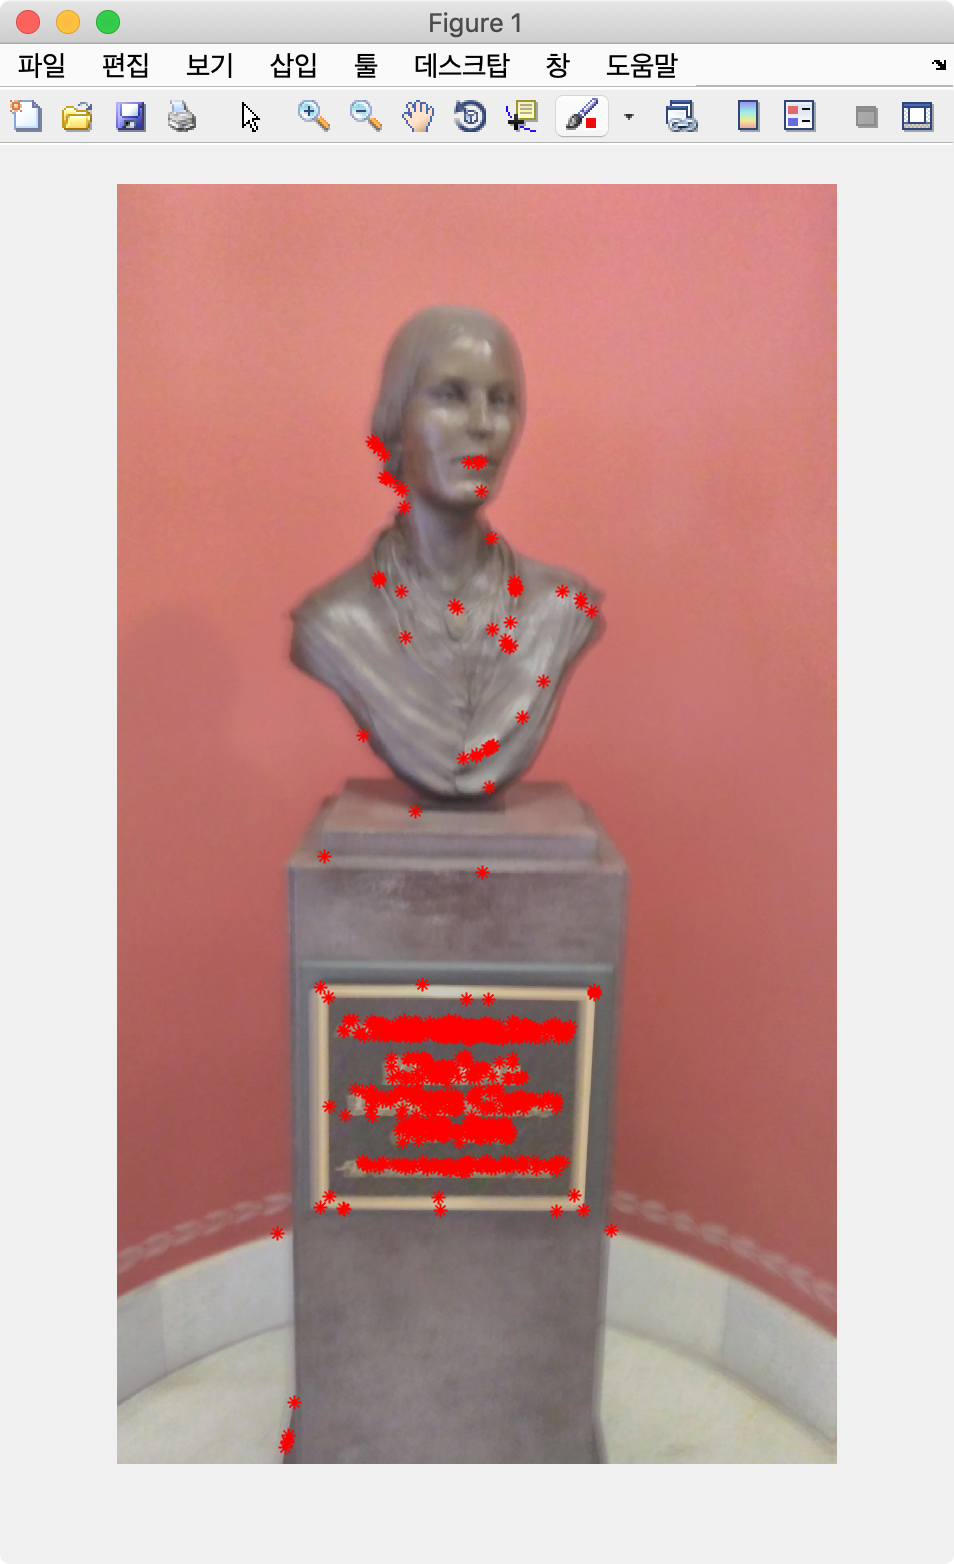
\includegraphics[width=3cm]{ch2.png}
  \caption{Result of \textit{Chase}}
  \label{fig:Chase}
\end{figure}

\begin{figure}[!hp]
  \centering
  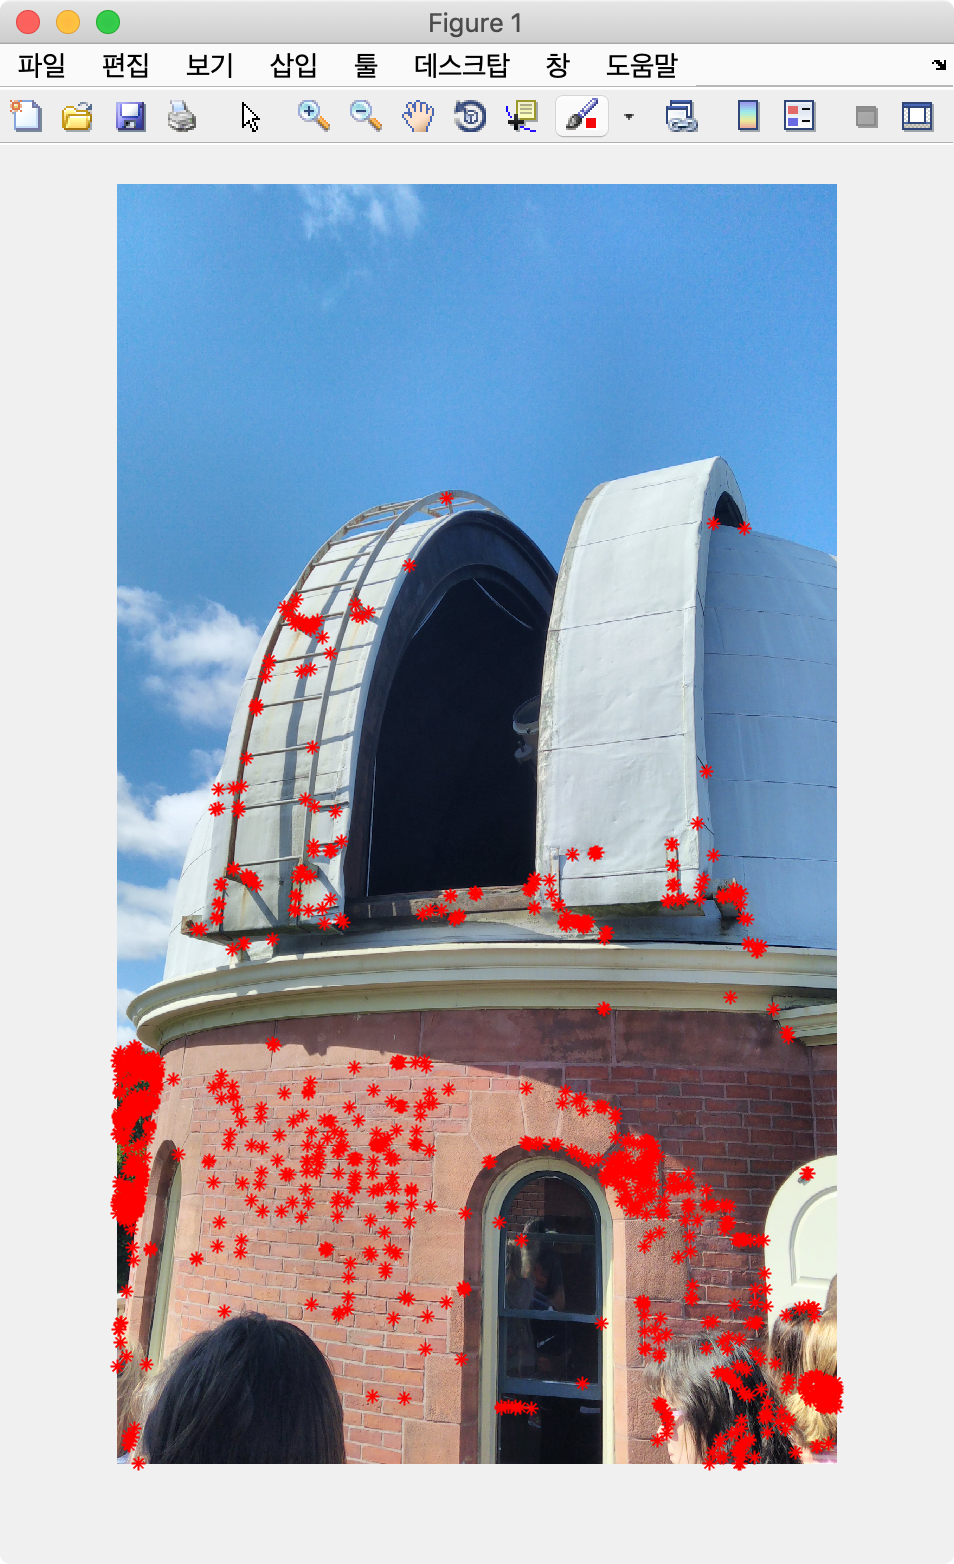
\includegraphics[width=3cm]{ob1.png}
  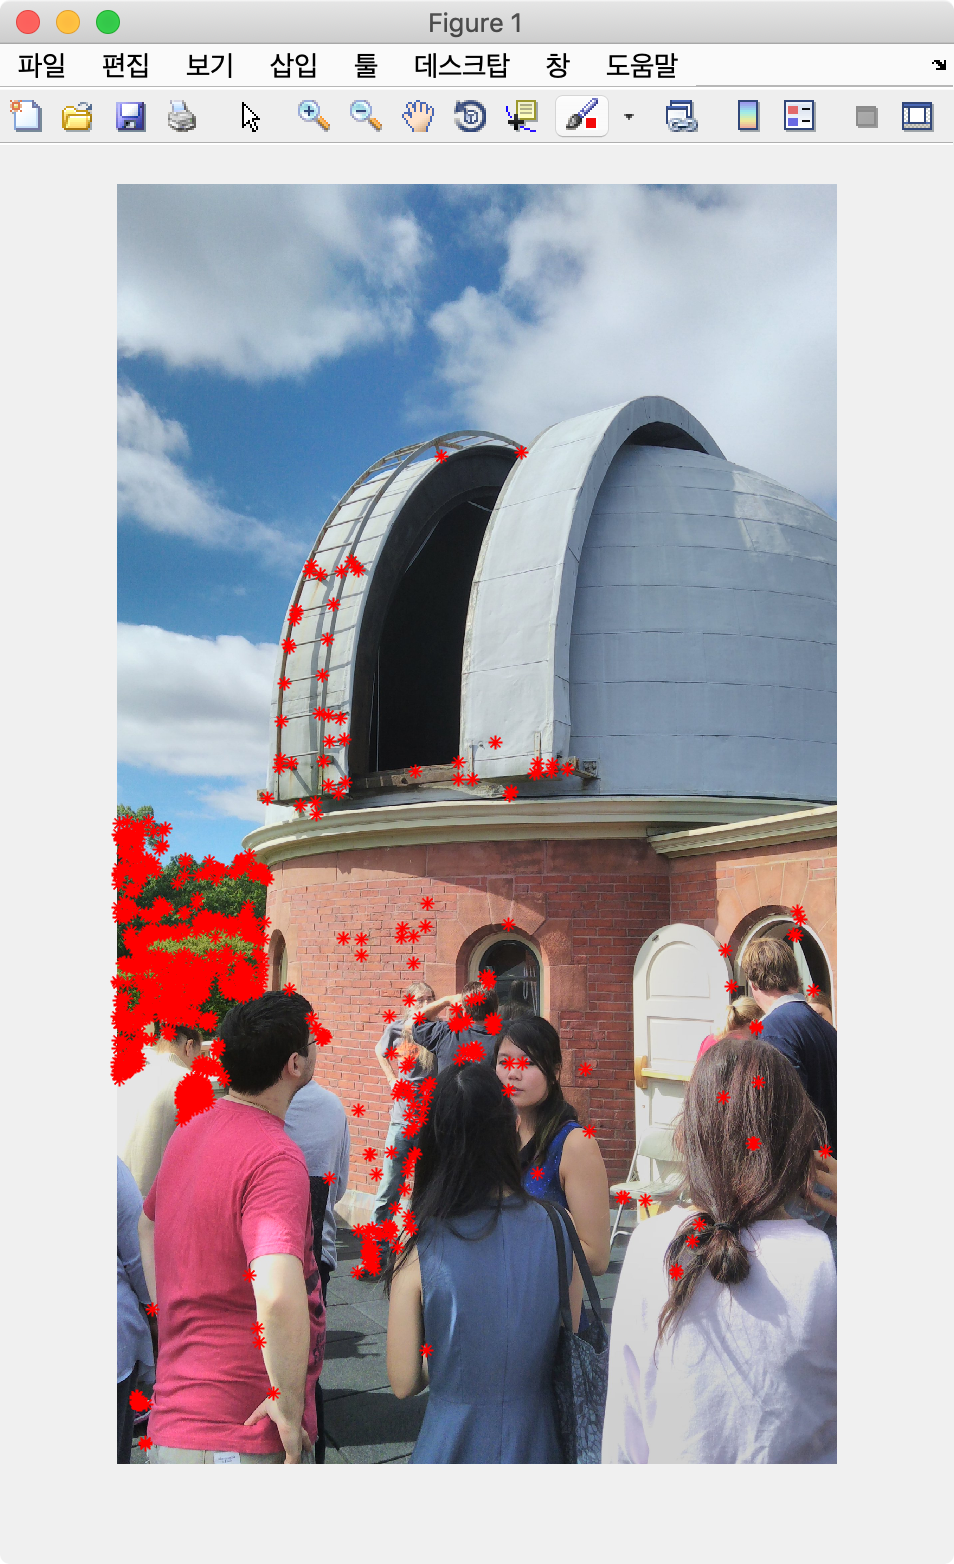
\includegraphics[width=3cm]{ob2.png}
  \caption{Result of \textit{LaddObservatory}}
  \label{fig:LaddObservatory}
\end{figure}

%%%%%%%%%%%%%%%%%%%%%%%%%%%%%%%%%%%

% Please leave the pagebreak
\pagebreak
\paragraph{Q2:} In designing our feature point, what characteristics might we wish it to have? Describe the fundamental trade-off between feature point invariance and discriminative power. How should we design for this trade-off?

%%%%%%%%%%%%%%%%%%%%%%%%%%%%%%%%%%%
\paragraph{A2:} The feature point should describe the significant point of the image. Invariance means which does not change during the transformation of the image. For example, rotation does not change the number of corners of the image.
Discriminative power means that how much pictures we can determine as different. So if we want strong invariance, the discriminative power will be decreased.

We should take care of those two terms carefully. We should keep our invariance in some necessary transformations -- such as tones of colors, rotations, and scaling.



%%%%%%%%%%%%%%%%%%%%%%%%%%%%%%%%%%%

% Please leave the pagebreak
\pagebreak
\paragraph{Q3:} In the Harris corner detector, what do the eigenvalues of the 'M' second moment matrix represent? Discuss both how they relate to image intensity and how we can interpret them geometrically.

%%%%%%%%%%%%%%%%%%%%%%%%%%%%%%%%%%%
\paragraph{A3:} The both eigenvalues represent the ellipses' two radius. The ellipses describe the gradient of the image.
If both values are big enough and have similar values, it means that the difference in pixels are huge in both directions. So it should be determined as corner.
If one value is much smaller than the another, it means that the difference occurs in only one direction -- it's edge.
It two values are not big enough, the point could be treated as flat.



%%%%%%%%%%%%%%%%%%%%%%%%%%%%%%%%%%%


% Please leave the pagebreak
\pagebreak
\paragraph{Q4:} Explain the difference between the Euclidean distance and the cosine similarity metrics between descriptors. What might their geometric interpretations reveal about when each should be used? Given a distance metric, what is a good method for feature descriptor matching and why?

%%%%%%%%%%%%%%%%%%%%%%%%%%%%%%%%%%%
\paragraph{A4:} Euclidean distance is the norm value between two vectors: $ || A - B || $.

Howerver, cosine similarity uses consine value between two vectors to define how much closer two vectors are. It is described as $ \frac{A \cdot B}{||A|| ||B||} $.

Using the NNDR (Nearest Neighbor Distance Ratio) method would be useful when a distance metric is given. NNDR method calculated the ratio between first-neighbor distance and the second-neighbor distance.
If the ratio is small enough, we could get more confidence for feature descriptor matching.

%%%%%%%%%%%%%%%%%%%%%%%%%%%%%%%%%%%


% If you really need extra space, uncomment here and use extra pages after the last question.
% Please refer here in your original answer. Thanks!
%\pagebreak
%\paragraph{AX.X Continued:} Your answer continued here.



\end{document}